\section{Methodology}
We compared the diffusion method against four DA methods and the baseline method without augmentation.
Figure \ref{fig:SystemDiagram} shows how the training sets were obtained using different combinations of the DA method and sampling size.
The sampling size was chosen at the ratio of 25, 50, 75, 100\%.
Five commonly used models for MI classification were used.
The models were trained using a subject-dependent scheme and evaluated on their respective testing sets. 

\begin{figure}[ht]
  \centering
  \caption[System Diagram]{\label{fig:SystemDiagram} Showed how to obtain training sets when using traditional DA and \texttt{WaveGrad}. \texttt{WaveGrad} was trained for each EEG channel in each class for each subject. Thus, we trained a total of 792 models from four classes, 22 channels and 9 subjects.}
  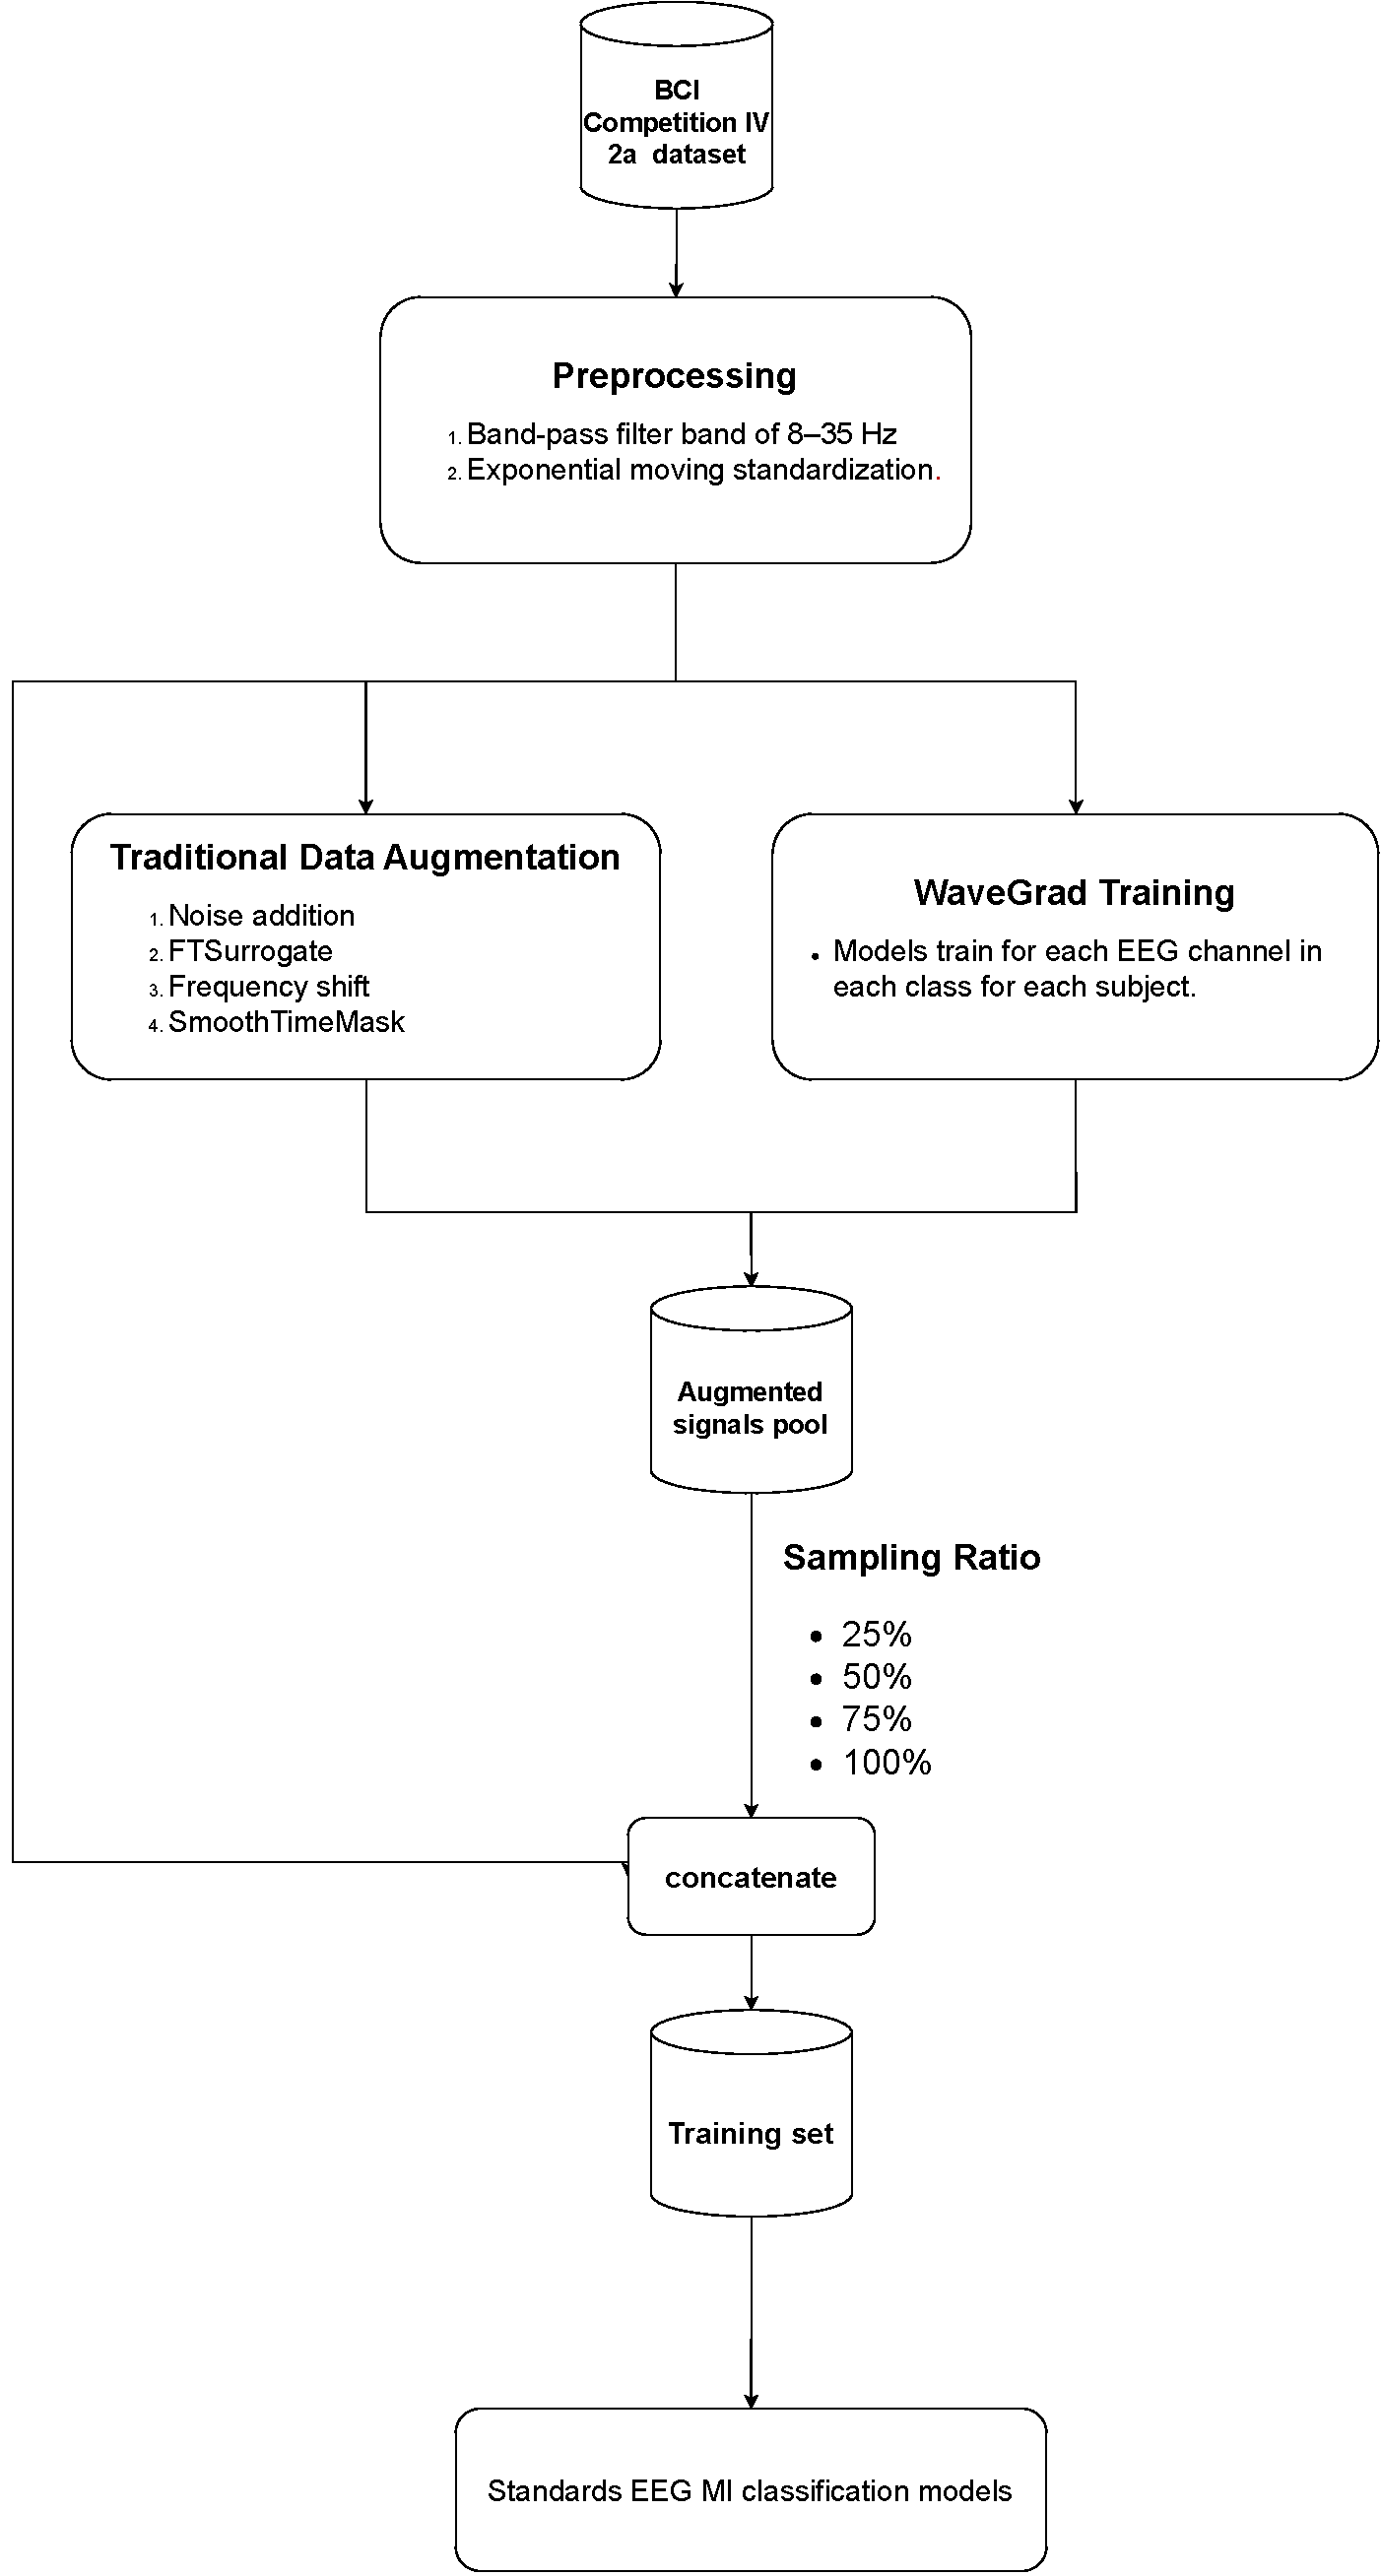
\includegraphics[width=0.6\textwidth]{fig/dyagram.pdf}
  \label{fig:System}
\end{figure}


\subsection{Datasets}
BCI Competition IV 2a \cite{brunner2008bci} was a collection of EEG data from 9 subjects who participated in a cue-based BCI paradigm involving four distinct motor imagery tasks: imagining movement of the left hand (class 1), the right hand (class 2), both feet (class 3) and the tongue (class 4).
Each subject completed the tasks in two distinct sessions on different days, with each session consisting of six runs separated by brief pauses, resulting in a total of 48 trials (12 for each of the four classes).
The data were captured while the participants sat in a comfortable armchair in front of a computer screen, and a fixation cross appeared at the start of each trial.
A cue consisting of an arrow pointing to the left, right, down, or up was used to prompt the subjects to perform the desired motor imagery task.
The subjects were instructed to perform the motor imagery task until the fixation cross disappeared from the screen without receiving any feedback.
Signals were sampled at 250 Hz and filtered between 0.5 Hz and 100 Hz using a 50 Hz notch filter to reduce line noise.
We used one section for training sets and another for test sets.

\subsection{Data Preprocessing}
EEG signal was filtered with a bandpass filter of 8 - 35 Hz followed by exponential moving standardization from \texttt{Braincode} library.

For exponential moving standardization, we computed the exponential moving mean $m_{t}$ at time $t$ as shown in equations (\ref{eq1}).
Then, we computed the exponential moving variance $v_{t}$ at time $t$ as shown in equation (\ref{eq2}).
Finally, we standardized the data point $x_{t}$ at time $t$ with $\alpha$ as 0.001 and $\epsilon$ as 0.0001 as shown in equation (\ref{eq3}).

\begin{eqnarray} 
m_{t} = \alpha \cdot \bar{x_{t}} + (1 - \alpha) \cdot m_{t-1}, \label{eq1}\\
v_{t} = \alpha\cdot (m_{t} - x_{t})^{2} + (1 - \alpha) \cdot v_{t-1} , \label{eq2} \\ 
x^{\prime}_{t} = \frac{(x_{t}-m_{t})}{\max(\sqrt{v_{t}},\epsilon), \label{eq3} }
\end{eqnarray}


\subsection{Data Augmentation}
Our objective was to assess the performance of each DA method with different ratios of augmented/synthetic data.
Five DA methods (\texttt{Noise Addition}, \texttt{FTSurrogate}, \texttt{Frequency Shift}, \texttt{SmoothTimeMask}, \texttt{WaveGrad}) and four ratios (25\%, 50\%, 75\%, 100\%) = 20 combinations (5 methods x 4 ratios) of the training set are to be created.
Here, ratios refer to the amount of augmented/synthetic data used.
For example, given a 25\% ratio, 25\% augmented data is randomly sampled and added to the original training set.
By comparing different ratios, we can better understand the impact of the size of augmentations on accuracy improvement.

Similar to previous works \cite{rommel2021cadda,mohsenvand2020contrastive,leeb2008bci,terzano2001atlas}, we used the subject-dependent scheme which augments data in subject level (i.e., each subject is treated separately) and channel level (i.e., each channel is treated independently).


\subsubsection{Noise Addition:}
\texttt{Noise Addition} entails the inclusion of diverse forms of noise, such as Gaussian, Poisson, and others, that possess varying parameters to the original EEG signal. 
The raw EEG signal was subjected to additive noise by incorporating a Gaussian distribution with a standard deviation of 0.1. 

\subsubsection{Fourier Transform Surrogates:}
\texttt{Fourier transform surrogates} are a type of data generated by randomizing the phases of temporal-spatial data.


\subsubsection{Frequency Shift:} The technique of \texttt{Frequency Shift} is characterized by the alteration of the frequency of the EEG signal by a specific amount.
We random shift the frequency by \textpm2 Hz.

\subsubsection{SmoothTimeMask:}
\texttt{SmoothTimeMask} involves applying a smooth window function to mask a continuous segment of the signal and optimizing it using gradient-based methods.
The signal was randomly masked with a range of 100 sample points.

\subsubsection{WaveGrad:}
It is first important that \texttt{WaveGrad} is originally a generative model, not a formal augmentation technique.
Thus, contrary to other DA methods, \texttt{WaveGrad} has to be trained before it can be used to generate a synthetic EEG signal.
The dataset consists of 9 subjects and four MI classes.
The EEG recording has 22 channels.
Thus, the total number of \texttt{WaveGrad} models was (9 subjects x 22 channels x 4 classes) = 792 models.
The training procedure and parameters were the same across all \texttt{WaveGrad} models.
The learning rate was set to 0.0001 and the diffusion steps to 1000.
\textcolor{red}{talk more about what you add/modify}

\subsection{Evaluation}
First, it is important to evaluate the quality of the augmented/synthetic data.
A common way is through dimensionality reduction KL divergence.
The success of the diffusion method in comparison to other methods is demonstrated by the Kullback-Leibler (KL) divergence, which is used to measure the similarity between the training set (with and without augmentation) and the validation set.
We expect that high-quality augmented or synthetic data should exhibit similarity between the training set (with and without augmentation) and the validation set.

Second, once the quality of the augmented/synthetic data is quantified, we are now ready to quantify the usefulness of data augmentation techniques on actual EEG tasks.
We first selected five commonly used motor imagery classification models (EEGNet, ATCNet, EEG-ITNet, Deep ConvNet and ShallowFBCSPNet) which would allow us to understand how the complexity of the model relates to data augmentation.
Here, note that we simply define the complexity based on the model's number of parameters.
Accuracy was then measured across all 21 combinations (5 DA methods x 4 sampling ratios + 1 baseline method without augmentation).
The details of each model were as follows:

\subsubsection{EEGNet}
%\textcolor{red}{intuition and parameters}
EEGNet is a single CNN architecture that can accurately classify EEG signals from different BCI paradigms while being as compact as possible.
The authors introduced the use of depthwise and separable convolutions to construct an EEG-specific model that encapsulates well-known EEG feature extraction concepts for BCI.
They compared EEGNet to current state-of-the-art approaches across four BCI paradigms and showed that EEGNet generalizes across paradigms and achieves comparably high performance when only limited training data is available across all tested paradigms.

\subsubsection{ATCNet}
%\textcolor{red}{intuition and parameters}
ATCNet was initially developed for predicting the onset of epileptic seizures using electroencephalogram (EEG) signals.
The ATCNet consists of two blocks: an attention-based temporal convolutional (ATC) block and a transformer-based classification (TC) block.
The ATC block is used to extract relevant features from the EEG signals, while the TC block is used to classify the extracted features into seizure and non-seizure classes.
The proposed model was evaluated using the BCI Competition IV-2a (BCI-2a) dataset.
The obtained accuracy ranged from 60.5\% to 89.5\%.

\subsubsection{EEG-ITNet}
EEG-ITNet uses inception modules and causal convolutions with dilation to extract rich spectral, spatial, and temporal information from multi-channel EEG signals with less complexity than other existing end-to-end architectures. 
The paper also provided a methodology for achieving intuitive visualization structures such as topographic maps.
The proposed EEG-ITNet model showed up to a 5.9\% improvement in classification accuracy compared to its competitors in different scenarios.

\subsubsection{Deep ConvNet}
The deep ConvNet had four convolution-max-pooling blocks, with a special first block designed to handle EEG input, followed by three standard convolution-max-pooling blocks and a dense softmax classification layer.
The authors found that recent advances in machine learning, including batch normalization and exponential linear units, together with a cropped training strategy, boosted the Deep ConvNets decoding performance, reaching at least as good performance as the widely used filter bank common spatial patterns (FBCSP) algorithm.

\subsubsection{ShallowFBCSPNet}
The shallow ConvNet is similar to the transformations of FBCSP.
Concretely, the first two layers of the shallow ConvNet perform a temporal convolution and a spatial filter, as in the deep ConvNet.
These steps are analogous to the bandpass and CSP spatial filter steps in FBCSP.